%%%%%%%%%%%%%%%%%%%%%%%%%%%%%%%%%%%%%%%%%
% University/School Laboratory Report
% LaTeX Template
% Version 3.1 (25/3/14)
%
% This template has been downloaded from:
% http://www.LaTeXTemplates.com
%
% Original author:
% Linux and Unix Users Group at Virginia Tech Wiki 
% (https://vtluug.org/wiki/Example_LaTeX_chem_lab_report)
%
% License:
% CC BY-NC-SA 3.0 (http://creativecommons.org/licenses/by-nc-sa/3.0/)
%
%%%%%%%%%%%%%%%%%%%%%%%%%%%%%%%%%%%%%%%%%

%----------------------------------------------------------------------------------------
%	PACKAGES AND DOCUMENT CONFIGURATIONS
%----------------------------------------------------------------------------------------

\documentclass{article}
\usepackage[margin=1in]{geometry}
%\usepackage[version=3]{mhchem} % Package for chemical equation typesetting
\usepackage{siunitx} % Provides the \SI{}{} and \si{} command for typesetting SI units
\usepackage{graphicx} % Required for the inclusion of images
%\usepackage{} % Required to change bibliography style to APA
\usepackage[backend=bibtex,maxnames=1]{biblatex}
\usepackage{amsmath} % Required for some math elements 
\usepackage{hyperref}
\usepackage{acronym}

%\usepackage[utf8]{vietnam}

\setlength\parindent{5pt} % Removes all indentation from paragraphs

%\renewcommand{\labelenumi}{\alph{enumi}.} % Make numbering in the enumerate environment by letter rather than number (e.g. section 6)

%\usepackage{times} % Uncomment to use the Times New Roman font

%----------------------------------------------------------------------------------------
%	DOCUMENT INFORMATION
%----------------------------------------------------------------------------------------

\title{Conditional Table Generative Adversarial Network:\\ On solving the problem of high cardinality} % Title

\author{\textsc{Anh-Dung} Dinh} % Author name

\date{\today} % Date for the report

\bibliography{sample}
\begin{document}

\maketitle % Insert the title, author and date
\newacro{AI}{Artificial Intelligence}
\newacro{GANs}{Generative Adversarial Networks}
\newacro{CTGAN}{Conditional Table Generative Adversarial Networks}
\begin{center}
\begin{tabular}{l r}
Supervisor: & Prof. Ngai-Man Cheung \\% Instructor/supervisor
& Dr. Ngoc-Trung Tran
\end{tabular}
\end{center}

% If you wish to include an abstract, uncomment the lines below
% \begin{abstract}
% Abstract text
% \end{abstract}

%----------------------------------------------------------------------------------------
%	SECTION 1
%----------------------------------------------------------------------------------------

\section{Introduction}

The problem of generating data has long attracted the great attentions from erudite scientists and scholars around the world. It could alternate traditional data, especially, when data is hard to achieve manually, and could provide adequate labels for training data as well instead of existing labelling data methods. This would result in extreme development in machine learning and \ac{AI} in the future due to its solution to the dearth of training data. In generative problems, one of very challenging and promising problems is to generate table data because of the seminal applications of synthetic table data. Usually, table data contains a lot of private information of users, businesses and governments. The publicity of this data, therefore, is impossible and dangerous which might confine researchers from doing experiments on this type of data. As a result, synthetic data is expected to keep the characteristics of the original data while keeping important information private. 

In general, there are a number of methods could help to produce synthetic data that is expected to match the distribution of the original data. Some of them are Bayesian methods [][], others are \ac{GANs} [][][]. Although \ac{GANs} could perform well on images as it learn the implicit distribution effectively, the performance of \ac{GANs} on table data is unexpectedly poor. The reason for this is that the table data often keep the mixture of continuous features and discrete features which are different from other homogeneous types of data such as images or texts. In order to solve this problem, a method has been proposed in [] which is named as \ac{CTGAN}. This method provides a modelling way for both discrete and continuous data based on one-hot vectors. The performance shown in the paper [] is better than other \ac{GANs}[][][] and Bayesian methods [][]. However, this input modelling method causes a very chronic problem which is high cardinality problem. If the number of features inside one column of the table data is too large, the one-hot vector becomes extremely long. As a result, the perennial mode collapse appears which facilitates the learning of "0" digits instead of the "1" digits due to the low frequencies of "1" digits. This causes poor performance for \ac{CTGAN} and need solving before this model could be applied in real-world problem as the real dataset often contains a lot of high cardinality features. In this work, we focus on solving the problem of high cardinality in table data generation. 

\section{Kiến thức cơ sở}\label{ktcs}

Về mặt chất lượng, yêu cầu quan trọng nhất của một sản phẩm là phải đáp ứng được đòi hỏi của khách hàng. Bên cạnh yêuyêu cầu từ phía người dùng, một số yêu cầu khác cũng cần được để tâm để đảm bảo sản phẩm được phát triển và bảo hành với chi phí tối thiểu. Nếu phần mềm cần được chỉnh sửa để trở thành một chương trình tổng quát (để có thể thay đổi tạo thành nhiều phần mềm khác nhau) thì lại còn phải đảm bảo thêm tính di động (portability). Nói chung, tính chất của một sản phẩm phần mềm có thể chia ra làm 3 loại là tính chất hoạt động, tính chất chuyển tiếp và tính chất sửa đổi.

Đối với tính hoạt động, một phần mềm cần phải đảm bảo được các tính chất sau:
\begin{itemize}
	\item \textit{Tính đúng đắn:} Phần mềm cần phải đảm bảo được các yêu cầu.
	\item \textit{Tính sử dụng được:} Thời gian hoặc nỗ lực để cho một người dùng có thể học cách sử dụng được phải thấp. Nói cách khác, giao diện người dùng cần phải thân thiện.
	\item \textit{Tính toàn diện:} Các hiệu ứng đi kèm cần được chỉnh chu.
	\item \textit{Tính hiệu quả:} Phần mềm cần phải sử dụng bộ nhớ một cách hợp lý hoặc tận dụng tài nguyên tính toán tốt.
	\item \textit{Tính tin cậy:} Phần mềm cần phải tránh được mọi hư hỏng trong quá trình vận hành.
	
	\item \textit{Tính an toàn:} Phần mềm không được làm ảnh hưởng tiêu cực đến môi trường hoặc cuộc sống con người xung quanh.
	\item \textit{Tính bảo mật:} Sản phẩm không được phép làm hư hại đến môi trường máy tính hoặc gây ảnh hướng xấu đến dữ liệu hoặc ổ cứng.
	\end{itemize}
	
	Tính chuyển tiếp là những yêu cầu về các mối liên quan đến các môi trường khác nhau đối với phần mềm:
	\begin{itemize}
		\item \textit{Tính linh động:} Phần mềm có thể chuyển và sử dụng được trên nhiều platform mà không ảnh hưởng đến chức năng. Ví dụ như phần mềm có thể hoạt động được trên cả windows và Unix.
		\item \textit{Tính tái sử dụng:} Một phần chức năng của phần mềm có thể sử dụng để xây dựng thành một phần mềm khác.
		\end{itemize}
		
	Tính chuyển đổi thì yêu cầu chương trình cần phải dễ dàng được thay đổi khi cần thiết:
	\begin{itemize}
		\item \textit{Tính thử nghiệm:} Chương trình cần phải dễ dàng kiểm thử.
		\item \textit{Tính nâng cấp:} Chương trình có thể mở rộng để phục vụ nhu cầu lớn hơn với chi phí nâng cấp có thể chấp nhận được.
		\item \textit{Tính mở rộng:} Sản phẩm cần phải dễ dàng được mở rộng thêm các chức năng nếu có yêu cầu.
		\item \textit{Tính phân tách:} Các phần của phần mềm nên được tách rời thành các phần độc lập. Điều này giúp cho việc quản lý, thay đổi hoặc kiểm thử dễ dàng hơn.
		\end{itemize}

	Các tính chất phần mềm được minh họa trong hình \ref{fig:characteristics}.
	
	\begin{figure}[h][h]
		\centering
		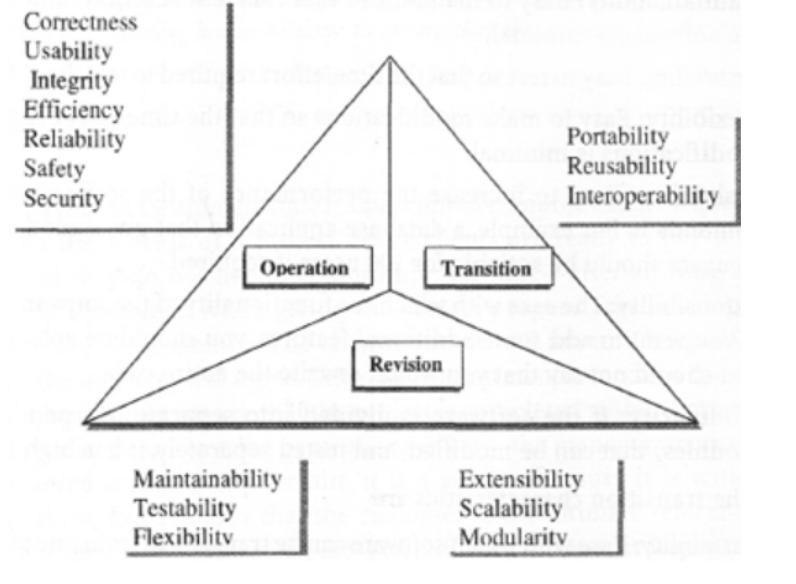
\includegraphics[scale=0.3]{figures/characteristics.png}
		\caption{Các tính chất của phần mềm}
		\label{fig:characteristics}
	\end{figure}
	
	Để đảm bảo các tính chât sphaanf mềm nói trên rất nhiều mô hình được sử dụng như là waterfall, V-shaped, evolutionary prototyping, iterative and incremental và agile. Ở phần này, em xin lược qua một số tính chất của các cách phát triển này.
	
	\subsection{Waterfall}
	
	Phương pháp waterfall hay thác nước là phương pháp cổ điển nhất. Phương pháp này được xem là một phương pháp SDLC (Linear Sequential Life Cycle Model) \cite{tutorialspoint}. Tức là phương pháp này được chia nhiều pha liên tục, mỗi pha phải được hoàn thiện trước khi bước vào pha sau. Minh họa các pha của waterfall được thể hiện ở hình 
	
	\begin{figure}[h]
		\centering
		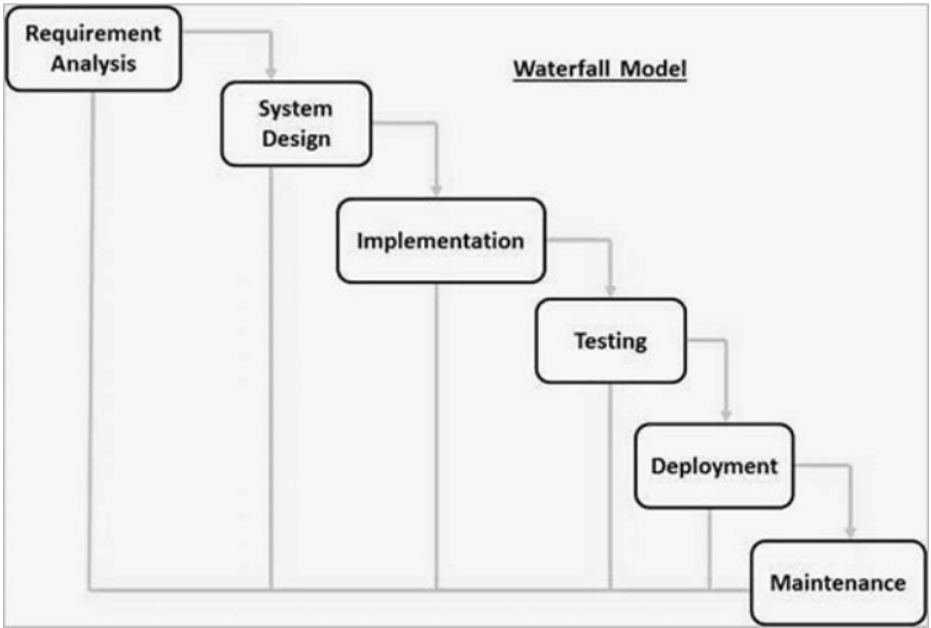
\includegraphics[scale=0.3]{figures/waterfall.png}
		\caption{Phương pháp waterfall \cite{tutorialspoint}}
		\label{fig:waterfall}
	\end{figure}
	
	Các pha của waterfall gồm:
	\begin{enumerate}
		\item \textit{Thu thập yêu cầu và phân tích:} Tất cả các yêu cầu của hệ thống đều phải được phân tích trong pha này và được lưu lại sử dụng cho các pha sau.
		\item \textit{Thiết kế hệ thống:} Mô tả của yêu cầu từ pha trước được phân tích trong pha này và bản thiết kế của hệ thống được vẽ ra. Bản thiết kế này giúp cho việc cụ thể hóa phần cứng, yêu cầu phần cứng và định hình cấu túcúc tổng quan của hệ thống.
		\item \textit{Thực hiện:} Với bản thiết kế có từ pha trước, ở pha này, hệ thống được phát triển thành các chương trình con gọi là các đơn vị. Mỗi hạng mục được phát triển và kiểm thử chức năng gọi là kiểm thử đơn vị (unit test).
		\item \textit{Tổng hợp và kiểm thử:} Tất cả các đơn vị phát triển từ pha trước được ghép lại ở pha này tạo nên một hệ thống sau khi kierm thử. Sau đó hệ thống được kiểm tra để phát hiện lỗi và đảm bảo hoàn thiện các chức năng.
		
		\item \textit{Triển khai:} Khi tất cả các chức năng được hoàn thiện và kiểm thử. Sản phẩm được triển khai trên môi trường yêu cầu bởi khách hàng và tung ra thị trường.
		\item \textit{Bảo trì:} Có rất nhiều vấn đề phát sinh sau khi triển khai. Để sửa các lỗi liên quan, các patch được phát hành để nâng cao chất lượng sản phẩm.		
		\end{enumerate}
		
	Điểm yếu của waterfall chính là các pha phải thực hiện tuần tự làm cho quá trình phát triển thiếu linh hoạt. Sản phẩm không có tính linh hoạt cao. Ngoài ra quá trình thiết kế đòi hỏi phải có rất nhiều kinh nghiệm để phân tích các rủi ro và ước lượng độ phức tạp của công việc.

% If you have more than one objective, uncomment the below:
%\begin{description}
%\item[First Objective] \hfill \\
%Objective 1 text
%\item[Second Objective] \hfill \\
%Objective 2 text
%\end{description}

\subsection{V-shaped}
\label{V-shaped}

V-shaped là một SDLC mà trong đó các bước thực hiện của quá trình được thực hiện theo hình chữ V đối xứng. 2 cánh của chữ V là Verification (xác thực) và Validation (kiểm tra). Hai cánh chữ V được nối bằng quá trình lập trình ở giữa. Hình minh họa cho mô hình V-shaped ở hình \ref{fig:vshape}. 


\begin{figure}[h]
	\centering
	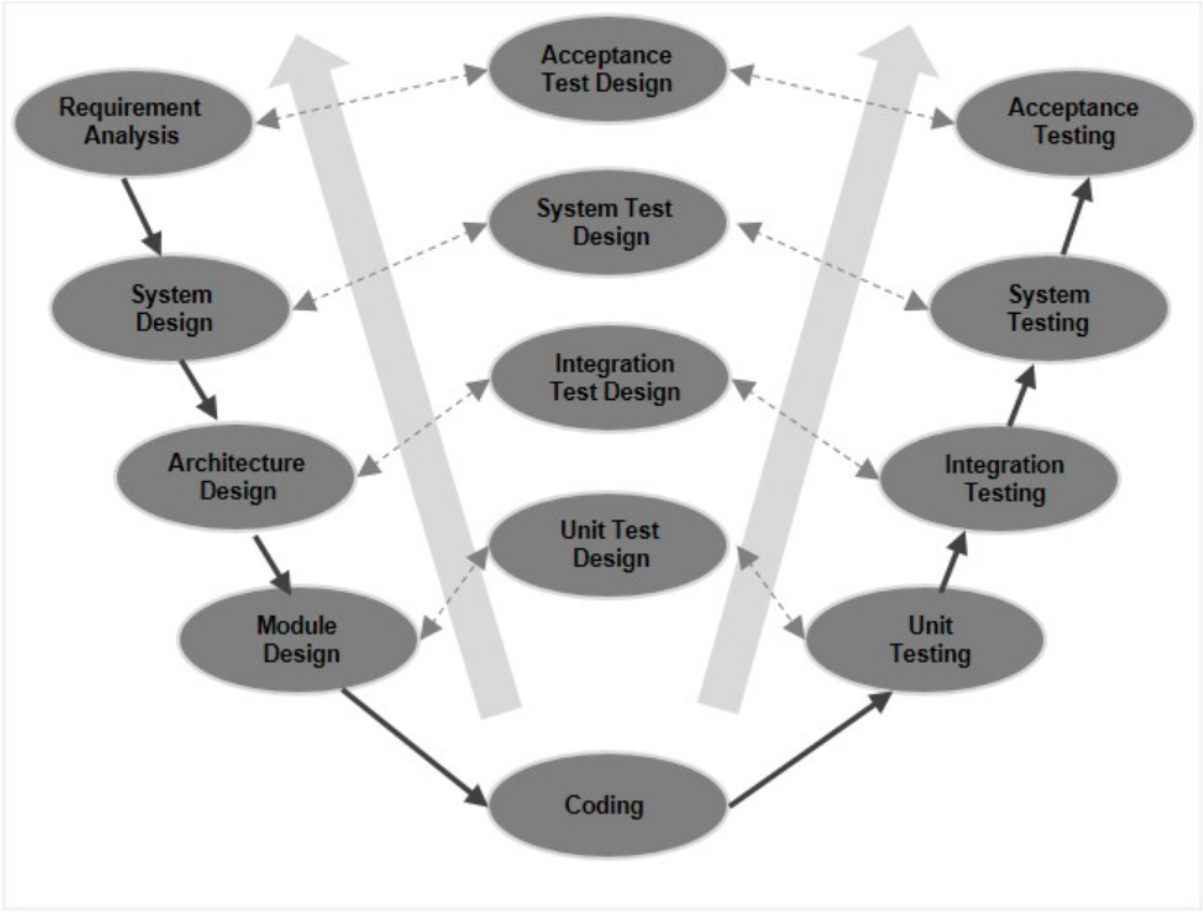
\includegraphics[scale=0.3]{figures/vshape.png}
	\caption{Phương pháp V-shaped \cite{tutorialspointvs}}
	\label{fig:vshape}
\end{figure}

v-shapedaped hoạt động tương đối giống với waterfall. Các bước xác thực và kiểm tra được thêm vào để đảm bảo sự rõ ràng trong kiểm thử phần mềm giúp cho phần mềm được hoạt động tốt hơn.

Tương tự như waterfall, V-shaped cũng gặp các vấn đề tương tự về tính linh hoạt của sản phẩm.

\subsection{Spriral}

Spiral có 4 pha. Một dự án phần mềm phải llawpj đi lặp ạiại các vòng lặp gọi là spiral gồm 4 pha này (Minh họa ở hình \ref{fig:spiral}).

\begin{figure}[h]
	\centering
	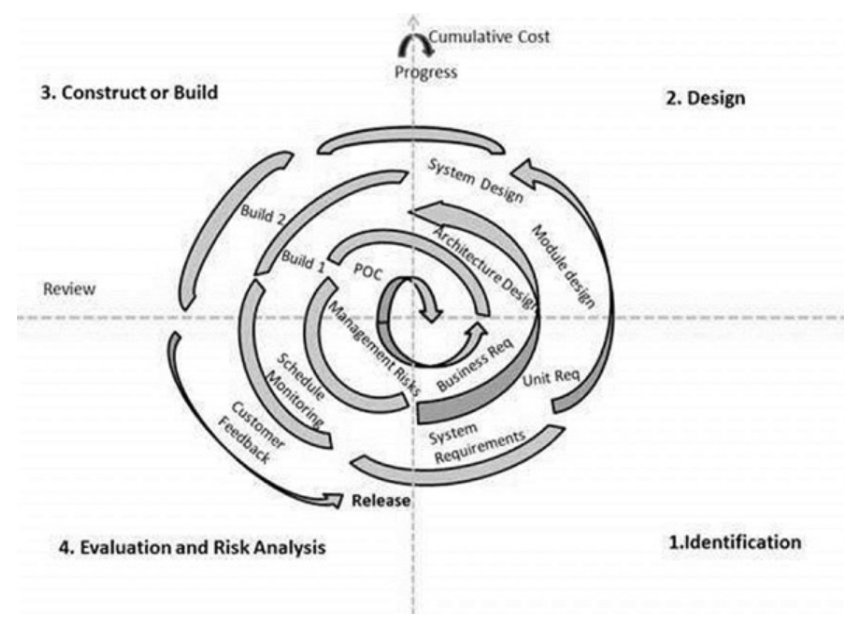
\includegraphics[scale=0.3]{figures/spiral.png}
	\caption{Phương pháp Spiral \cite{tutorialspointsp}}
	\label{fig:spiral}
\end{figure}


\begin{enumerate}
	\item \textit{Xác định:} Pha này bắt đầu bằng việc thu gom các yêu cầu từ khách hàng làm cơ sở chính cho spiral. Yêu cầu sản phẩm, yêu cầu hệ thống, yêu cầu của các hệ thống con và yêu cầu cho từng đơn vị đều được đưa ra trong pha này. Ở pha này, các yêu cầu hệ thống cũng được liên tục thảo luận với khách hàng và chuyên viên phân tích hệ thống. Đến cuối spiral, hệ thống được triển khai trên môi trường này. 
	
	\item \textit{Thiết kế:}  Sau khi có mô tả của các yêu cầu, thiết kế của hệ thống sẽ được chi tiết hóa bao gồm kiến trúc hệ thống, thiết kế các mô-đun và thiết kế các spirals.
	
	\item \textit{Xây dựng:} Đây là khâu hiện thực hóa bản thiết kế trước đó. Dựa vào phản hồi của khách hàng về thiết kế, sản phẩm được thiết kế mẫu rồi tiếp tục lấy đánh giá của khách hàng. Các spiral quan trọng được phát triển theo các phiên bản rồi liên tục lấy đánh giá của khách hàng rồi tiếp tục phát triển. 
	
	\item \textit{Đánh giá và phân tích rủi ro:} Phân tích rủi ro bao gồm xác định, đánh giá và giám sát các trường hợp bất khả kháng liên quan đến quản lý và kỹ thuật giống như là trễ thời hạn hoặc đội vốn, đội giá. Sau chu trình đầu tiên, khách hàng sẽ được lấy ý kiến và sản phẩm tiếp tục được phát triển dựa theo ý kiến của khách hàng. 
	\end{enumerate} 


\section{Hệ thống phương pháp Agile}

Hệ thống phương pháp agile là một hướng tiếp cận để quản lý cho các dự án phát triển phần mềm. Phương pháp này giúp cho đội phát triển phản ứng lại với các sự cố trong quá trình xây dựng phần mềm. Theo đó, phương pháp này sử dụng các bước lặp lại và gia tăng giống như trong sprint đã trình bày ở mục \ref{ktcs}. 

Agile được dịch ra tiếng Việt có nghĩa là nhanh nhẹn. Bản thân agile không phải là một cách thức để phát triển phần mềm mà là mục tiêu cần đạt được. Chính vì vậy agile không phải là một phương pháp mà chỉ là một cách tiếp cận để quản lý quá trình phát triển phần mềm để đảm bảo cả về mặt chất lượng lẫn thời gian \cite{wisdomjobs}. Cụ thể hơn, phát triển theo hướng agile có nghĩa là:
\begin{itemize}
	\item \textit{Tăng cường sự tham gia của khách hàng:} Quá trình truyền thống thường chỉ cho phép khách hàng tham gia vào phần đầu lúc đưa ra yêu cầu chi tiết và phần cuối lúc nghiệm thu và triển khai sản phẩm. Trong agile, mỗi hạng mục đều cần phải có sự phản hồi của khách hàng, nhờ vậy phần mềm đưa ra gần như tiệm cận với mong muốn của khách hàng. Điều này là một điểm nâng cao rất lớn so với quá trình phát triển truyền thống, quá trình truyền thống có thể khiến cho đội phát triển đưa ra một sản phẩm khách hoàn toàn với mong muốn của khách hàng, nguyên nhân có thể là do phân tích sai yêu cầu, có thể là do không hiểu đúng mon muốn của khách hàng. Tuy nhiên, những tác nhân đó đều có thể giải quyết nếu khách hàng cùng tham gia vào quá trình phát triển và phản hồi nhận xét thường xuyên.
	
	\item \textit{Nâng cao tính ưu tiên của các tính năng:} Các quá trình agile nâng cao tính ưu tiên và đưa ra các tính năng với giá trị cao trươc.s Điều này có thể đạt được bằng cách tạo các thẻ tính năng (feature cards) hoặc vẽ ra các trường hợp người dùng (user stories) và đánh giá tính năng đó trước khi yêu cầu chi tiết được đưa ra. Nhóm phát triển sẽ giúp khách hàng của mình đánh giá được giá trị, rủi ro, tần suâts sử dụng và tính độc lập của tính năng giúp cho:
	\begin{itemize}
		\item Ước tính lượng công việc à đánh giá rủi ro sớm trong quá trình phát triển.
		\item Ưu tiên những tính năng có giá trị cao được phát triển sớm trong quá trình.
		\item Đưa ra các tính năng độc lập nhau. 
		\end{itemize}
	Theo đó, độ ưu tiên của tính năng trong agile giúp cho đội ngũ phát triển hoạt động trơn tru hơn và tạo được sản phẩm vượt qua được ác bài test thử ưu tiên. 
	
	\item \textit{Tăng cường độ tham gia của các cá nhân trong đội ngũ phát triển:} Phần lớn mọi người tỏng dự án agile được tham gia vào quá trình lên kế hoạch, ước tính và lập lịch. Cả đội cũng tham gia vào các quá trình này lặp đi lặp lại. Qua thời gian, các thành viên trong đội sẽ dần có ý tưởng đóng góp vào các chức năng trong sản phẩm. Từ đó tăng độ tích cực của các thành viên trong nhóm và đảm bảo mọi người hiểu nhau hơn và hiểu giá trị của dự án trước khi công việc bắt đầu và tăng động lực cho các thành viên trong đội ngũ.
	
	\item \textit{Làm rõ độ ưu tiên và nhắc nhở mọi người về những hậu quả nếu thay đổi:} Một đội agile làm việc với khách hàng hoặc các bên liên quan để xác định các vấn đề cốt yếu trong dự án như ngân sách, độ ưu tiên của chức năng. Đội này sẽ học được thứ tự ưu tiên và sử dụng kiến thức này để ra quyết định chọn lựa chi phí cơ hội trong quá trình phát triển sản phẩm.
	
	\item \textit{Thích ứng với sự thay đổi:} Một phương pháp agile cho phép đánh giá lại hoặc chuyển hướng dự án trong quá trình phát triển hoặc hoạt động. Nhóm phát triển thực hiện các bước theo các chu trình và demo sản phẩm ở cuối mỗi chu trình. Khách hàng có thể kiến nghị thay đổi ở mỗi chu trình. Dù điều này có thể ẩn chứa các rủi ro trong tương lai nhưng đội phát triển có thể đáp ứng được mọi đòi hỏi của khách hàng. 
	
	\item \textit{Hiểu hơn về trạng thái của dự án:} Phát triển agile là phát triển theo kiểu đóng khung thời gian. Đội phát triển đánh giá trạng thái bằng cách biểu diễn hoạt động của các chức năng. Các task bổ trợ cũng được đánh giá ở dạng binary (hoàn thành hoặc không hoàn thành) để loại trừ các nhầm lẫn khi biểu thị bằng phần trăm khối lượng hoàn thành. Một quá trình agile cũng bao gồm các thành viên phải báo cáo trạng thái công việc của họ với quản lý hoặc bên liên quan. Điều này nâng cao tính chính xác và trách nhiệm cảu mỗi cá nhân.
	
	\item \textit{Lên kế hoạch tốt hơn:} Rất nhiều công ty cố gắng lên kế hoạch chi tiết từ khi dự án khởi động. Kế hoạch dù chi tiêts cũng sẽ ẩn chứa nhiều yếu tố khách quan không thể quyết định trước. Trong khi đó, đội phát triển theo hướng agile đưa ra kế hoạch tổng quan, còn độ chi tiết của kế hoạch sẽ được thảo luận dựa trên độ thiếu chắc chắn của các yếu tố khác.
	
	\item \textit{Liên tục kiểm soát rủi ro:} Đây là một điểm mạnh của cách tiếp cận này. Các quá trình phát triển luôn muốn đội phát triển phải luôn cập nhật thông tin tiến độ và thay đổi của dự án. 
	
	\item \textit{cung cấp tư liệu cần thiết ở cuối dự án:} Ý tưởng đằng sau một phương pháp agile đó là sự thiếu chắc chắn đối với rất nhiều yếu tố khách quan. Chính vì những yếu tốt khách quan này, các tư liệu như phân tích rủi ro, yêu cầu ở ngay đầu dự án sẽ trở nên lỗi thời và không hợp lý khi nghiệm thu. Như vậy, một phương pháp agile cần được sử dụng để luôn nhận biết sự thay đổi trong dự án từ đó định hình và thay đổi các tư liệu cần thiết để đảm bảo quá trình triển khai thành công. 
	
	\item \textit{Định hình đúng cấu trúc dự án:} Có rất nhiều công ty định ra được các quy trình và các chu trình để phát triển 1 dự án. Mỗi khi, một quản lý hay một lập trình viên không biết phải làm gì tiếp thì chỉ cần nhìn vào quy trình của công ty để làm tiếp. Việc này rất có lợi nếu như các thành viên trong đội ngũ phát triển thiếu kinh nghiệm. Tuy nhiên, một đội ngũ giàu kinh nghiệm thì sẽ biết những công việc nào là không cần thiết hoặc một số công đoạn có thể bỏ qua đối với các dự án cụ thể. Ép buộc những nhân viên này theo một khuôn khổ định sẵn sẽ gây ra sự đối phó đối với từng bước. Agile yêu cầu quy trình này phải thật gọn nhẹ và phải tùy thuộc vào tính chất của từng dự án. Từ đó, các thành viên trong đội phát triển có thể phát triển dựa vào kinh nghiệm của mình nhưng cũng tuân thủ được các yêu cầu của dự án. 
	\end{itemize}
	
\subsection{Các phương pháp Agile}

Như đã nói ở trên, agile là một hướng tiếp cận chứ bản thân không phải là phương pháp. Hiện có rất nhiều mô hình và phương pháp tuân thủ theo quy luật của agile. Trong đó có Scrum, Extreme programming (XP), ... Tùy thuộc vào tính chất của dự án thì nhà phát triển cần lựa chọn hướng đi phù hợp cho mình. 

\subsubsection{Scrum}

Scrum là quá trình bắt đầu bằng việc xác định các chức năng có độ ưu tiên cao nhất và ước tính số lượng chức năng để đưa vào 1 sprint. Các chức năng này được soạn thảo ra một thư mục sprint backlog. Một sprint tương ứng với 1 khoảng thời gian từ 2 đến 4 tuần bao gồm phân tích, thiết kế, xây dựng, thử nghiệm và soạn thảo hướng dẫn, đặc tả cho từng chức năng. Ảnh \ref{fig:scrum} minh hoạc quá trình này. 

\begin{figure}[h]
	\centering
	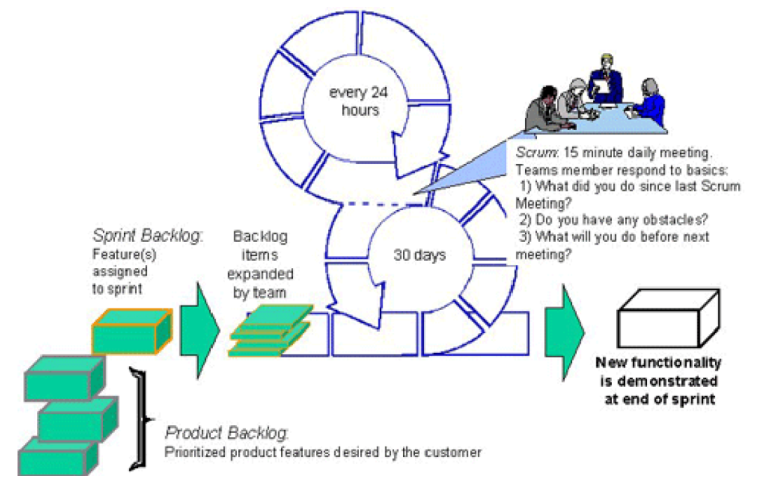
\includegraphics[scale=0.3]{figures/scrum.png}
	\caption{Phương pháp Scrum \cite{poccia1970}}
	\label{fig:scrum}
\end{figure}

Thường thì hằng ngày nhom sẽ phải họp để đánh giá trạng thái của dự án. Các cá nhân trong nhóm cần phải trả lời:
\begin{enumerate}
	\item Đã hoàn thành công việc được giao từ lần họp trước chưa?
	\item Sẽ làm gì trong ngày hôm nay?
	\item Những khó khăn gì gặp phải trong công việc trước đó?
	\end{enumerate}
	
	Khi một sprint được hoàn thành, các chức năng được biểu diễn cho khách hàng. Sau đó, độ phát triển và khách hàng quyết định xem công việc cần thêm vào là gì, hoặc quyết định xem sản phẩm đã có thể được xuất bản hay chưa. Qua mỗi sprint, công việc cần được đánh giá trên các hạng mục theo xu hướng tốt lên hoặc xấu đi. Kế hoạch sau đó sẽ được thảo ra để khắc phục những tồn đọng trước đó. 
	
	Từ đó để có được một quá trình làm scrum, thì các điều kiện cần đó là:
	\begin{itemize}
		
		\item \textit{Kỷ luật:} Scrum bám rất sát vào thời gian, công việc lập trình thường ngày và trách nhiệm của các thành viên trong nhóm. Không có kỷ luật công việc sẽ không thể đảm bảo tiến đến độ ngày và ảnh hưởng đễn cả công việc của toàn đội ngũ phát triển. 
		
		\item \textit{Nguyên tắc ba kiềng:} Một đội Scrum sẽ bao gồm ScrumMaster, nhà phát hành sản phẩm và nhân viên trong nhóm. Mỗi một trong các vị trí trên đảm bảo một phần về mặt chất lượng của sản phẩm. 
		
		\item \textit{Chất lượng:} Chức năng cần phải được hoàn thành toàn bộ và có thể triển khai được sau mỗi sprint. 
		\end{itemize}

	Từ đó ta có thể thấy được điểm mạnh của Scrum là:
	\begin{itemize}
		\item \textit{Triển khai theo ưu tiên:} Các chức năng được triển khai theo thứ tự tương ứng với giá trị tài chính.
		\item \textit{Không quy định cụ thể các bước trong mỗi sprint}
		\item \textit{Thực hiện thành công ở nhiều lĩnh vực phần mềm:} Scrum đã được thử và áp dụng thành công trong rất nhiều môi trường.
		
		\item \textit{Trạng thái minh bạch:} Trong suốt quá trình phát triển sản phẩm, trạng thái của sản phẩm luôn được công khai và có thể theo dõi được đối với mọi thành viên trong nhóm.
		
		\item \textit{Đóng góp toàn đội:} Mọi người trong đội ngũ phát triển và khách hàng đều có thể tham giá đóng góp vào quá trình phát triển sản phẩm giúp cho sản phẩm hoàn thiện hơn. 
		
		\item \textit{Liên tục hoàn thành:} Scrum luôn hoàn thành và đưa các chức năng, tính năng của sản phẩm một cách liên tục. 
		\end{itemize}

	Dẫu được mô tả là có nhiều điểm mạnh, bản thân Scrum vẫn tồn tại nhiều hạn chế:
	\begin{itemize}
		\item Scrum không có sự phân hóa chuyên môn mạnh. Điều này rất khó đối với một đội ngũ có mức độ phân hóa cao có thể được quản lý theo hướng Scrum vì thường trong Scrum tất cả mọi người thuộc đội ngũ đều có thể làm mọi việc miễn là việc đó có thể hoàn thành sprint. 
		
		\item Kết quả của một Scrum phụ thuộc rất lớn vào ScrumMaster.
		\item Do Scrum là một phương pháp tương đối tổng quan. Việc đưa ra quyết định trong mỗi thời điểm phải làm gì đòi hỏi các lập trình viên cần phải có rất nhiều kinh nghiệm. 
		\end{itemize}
		
	Hiện tại Scrum đang ngày càng phổ biến đến mức khi nhắc đến agile thì người ta sẽ nghĩ đến scrum. Phương pháp này cho thấy một quá trình lặp lại một cách tinh tế phù hợp với phats triển sản phẩm và quản lý các phiên bản. Để tìm hiểu về scrum, hiện cũng đã có rất nhiều tài liệu cụ thể có thể dùng để áp dụng vào thực tế. thêm vào đó, scrum vẫn cần các cách tiếp cận agile khách để hoàn thành các chu trình phát triển sản phẩm của mình.
	
	\subsubsection{Extreme programming}
	
	Tương tự như scrum, XP bắt đầu quá trình bằng cách tạo backlog cho công việc ở mỗi sprint. XP tạo ra backlog bằng cách thảo luận với khách hàng, tạo các trường hợp người dùng (user stories). Song song với đó, đội ngũ phát triển cũng tạo ra một kiến trúc spike, mà từ đó có thể thử giả định với các trường hợp khách nhau để định hình ra kiến trúc chương trình đầu tiên. XP gọi đây là khâu khai phá.
	
	Sau khâu khai phá thì sẽ đến khâu lên kế hoạch. Ở khâu này, các trường hợp người dùng quan trọng nhất được xác định và lên lịch bao giờ có thể hoàn thành. Các nhiệm vụ được định ra cho mỗi chức năng để có thể dễ dàng ước tính được độ phức tạp của công việc. Đội ngũ phát triển có thể tạo được một lịch trình tổng quan và có thể hình dung được các yếu tố không chắc chắn có khả năng xảy ra cao trước khi dự án bắt đầu. Một phiên bản có thể bao gồm nhiều vòng lặp và mất 2-4 tuần cho việc xây dựng.
	
	Khi một chu trình vòng lặp được bắt đầu, kế hoạch cho chu trình này được xem xét lại. Đội ngũ lúc này thêm vào các trường hợp người dùng và nhiệm vụ được phát hiện trong quá trình liệt kê trước đó.
	
	XP kết hợp vơi skhachs hàng trong quá trình kiểm thử ở mỗi chu trình vòng lặp. Mỗi khách hàng được hỏi về các tiêu chuẩn kiểm thử và đội phát triển sẽ đưa các tiêu chuẩn này vào máy tính để đảm bảo được phần mềm có thể vượt qua hết các bài kiểm tra chất lượng.
	
	Ngay sau khau lên kế hoạch thì ở khâu thực hiện, các mã nguồn được hoàn thành. Mã nguồn được kiểm tra để đáp ứng với nhu cầu của khách hàng cũng như các yêu cầu về mặt chức năng như là đảm bảo tải lượng, đảm bảo về dịch vụ và thời gian phản hồi của sản phẩm. Ảnh \ref{fig:xp} mổ tả XP.
	
		\begin{figure}[h]
			\centering
			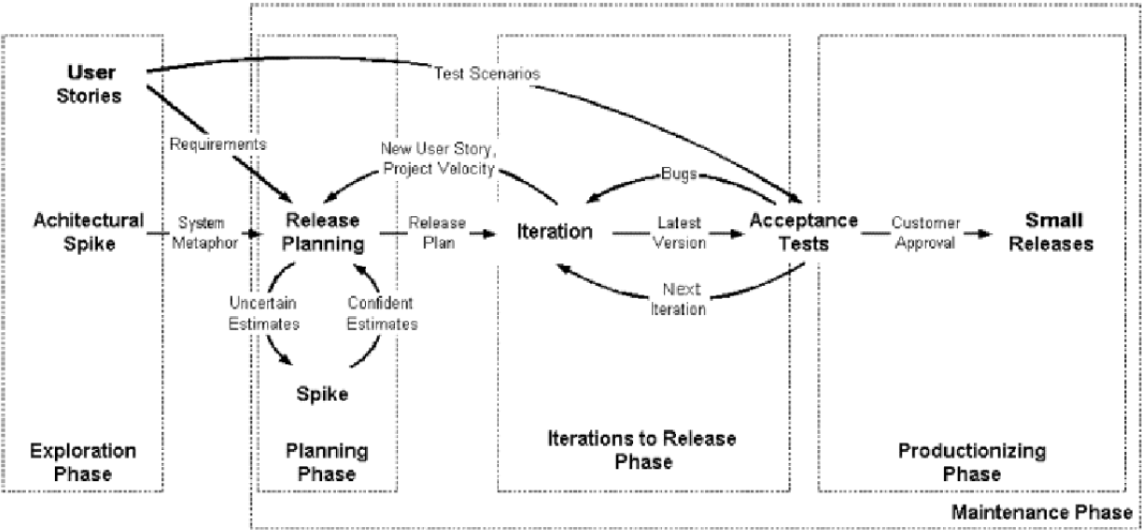
\includegraphics[scale=0.3]{figures/xp.png}
			\caption{Phương pháp Scrum \cite{poccia1970}}
			\label{fig:xp}
		\end{figure}
	
	Từ đó một số đặc tính của XP được rút ra như sau:
	
	\begin{itemize}
		\item \textit{Cụ thể:} Không giống như Scrum, XP cụ thể về mặt kỹ thuật để có thể sử dụng được trong suốt dự án phần mềm. Những kỹ thuật nào bao gồm lập trình theo cặp, TDD, liên tục tích hợp, tái định hình và gia tăng mã nguồn.
		
		\item \textit{Mô hình hóa:} Đội XP thường xuyên sử dụng mô hình hóa để hiểu hơn về nhiệm vụ cũng như kiến túc dự án để hoàn thiện các trường hợp người dùng.
		
		\item \textit{Đơn giản:} Đội ngũ chỉ cần làm việc đủ để đảm bảo được yêu cầu buổi họp.
		\item \textit{Tự động:} Các phương thức kiểm thử về các hạng mục được tự động hóa.
		
		\item \textit{Chất lượng thông qua kiểm thử:} Các chức năng luôn được kiểm thử thường xuyên và các lập trình viên kierm tra mã nguồn lẫn nhau thông qua lập trình theo cặp.
		\end{itemize}
	
	Điểm mạnh của XP:
	\begin{itemize}
		\item Tập trung vào khách hàng (tất cả đều xoanh quanh trường hợp người dùng).
		\item Chất lượng thông qua liên tục kiểm thử.
		\item Tập trung đặc biệt vào các chức năng quan trọng của sản phẩm.
		\item Tính minh bạch cao.
		\item Giúp cho đội phát triển thích ứng được với các yêu cầu biến đổi liên tục về chức năng..
		\end{itemize}
		
	Tuy nhiên, XP vẫn còn tồn tại nhiều hạn chế:
	\begin{itemize}
		
		\item  Cần đội ngũ có kinh nghiệm
		\item Phát triển độc lập với kiểm thử
		\item Chỉ phù hợp với các dự án nhỏ
		\item Phụ thuộc vào vị trí làm việc của các thành viên trong đội ngũ phát triển.
		\end{itemize}
		
	XP hỗ trợ rất nhiều mục tiêu quan trọng trong quá trình agile như là xử lý các vấn đề liên quan đến thay đổi yêu cầu, tính ưu tiên của chức năng. XP cũng tuân thủ theo triết lý tối giản tức giảm thiểu các công việc thừa thãi không cần thiết.
	
	XP nhiều lúc bị chỉ trích vì tính nguyên tắc trong quá trình thiết kế và viết tài liệu hệ thống. Trong những năm gần đây điều này có vẻ đã thay đổi, XP thường tạo ra tài liệu cần thiết hướng đến người dùng và khách hàng. 
	
\section{ Ứng dụng agile}

Trong phần này, em xin trình bày phần ứng dụng của agile vào một project cụ thể là xây dựng một trang web bán hàng. Để bắt đầu xây dựng chương trình, thì một thiết kế tổng quan về yêu cầu được đưa ra như trong biểu đồ usecase như hình \ref{fig:usecase}. Gồm có 5 modules, module xác thực, module sản phẩm, module quản lý sản phẩm, module quản lý người dùng và module đặt hàng và thanh toán. Do module sản phẩm, module xác thực và module đặt hàng thanh toán là 3 module chính của chương trình. 3 module này sẽ được xây dựng trước. 

\begin{figure}[h]
	\centering
	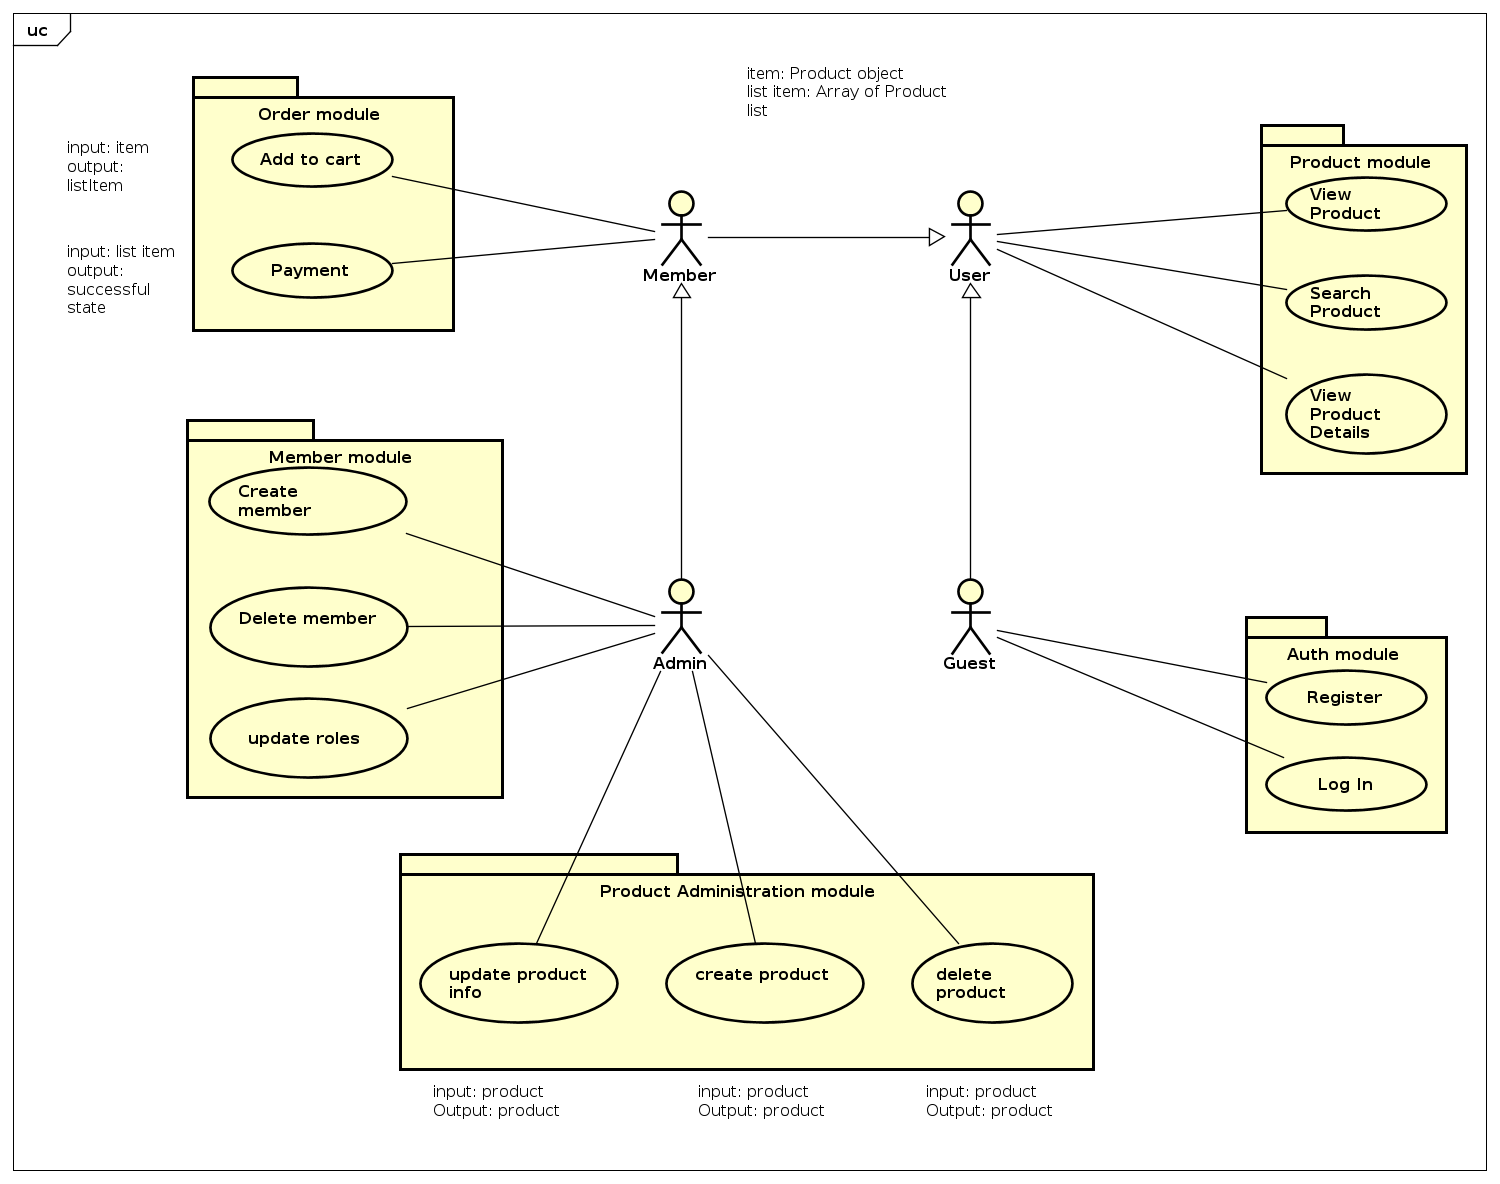
\includegraphics[scale=0.3]{figures/usecase.png}
	\caption{Biểu đồ usecase cho trang web bán hàng trực tuyến}
	\label{fig:usecase}
\end{figure}


\subsection{Sprint 1: Xây dựng module xác thực}

Module này yêu cầu người dùng đăng ký để có tài khoản thành viên. Trước tiên, để lưu trữ được thông tin người dùng thì cơ sở dữ liệu cho người dùng cần được xây dưng. Cơ sở dữ liệu cho người dùng được xây dựng như bảng \ref{fig:datareg}

\begin{figure}[h][h]
	\centering
	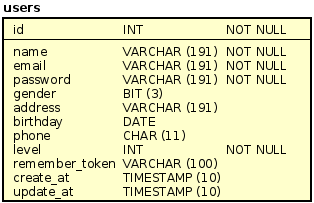
\includegraphics[scale=0.3]{figures/datareg.png}
	\caption{Cơ sở dữ liệu người dùng}
	\label{fig:datareg}
\end{figure}

\begin{figure}[h]
	\centering
	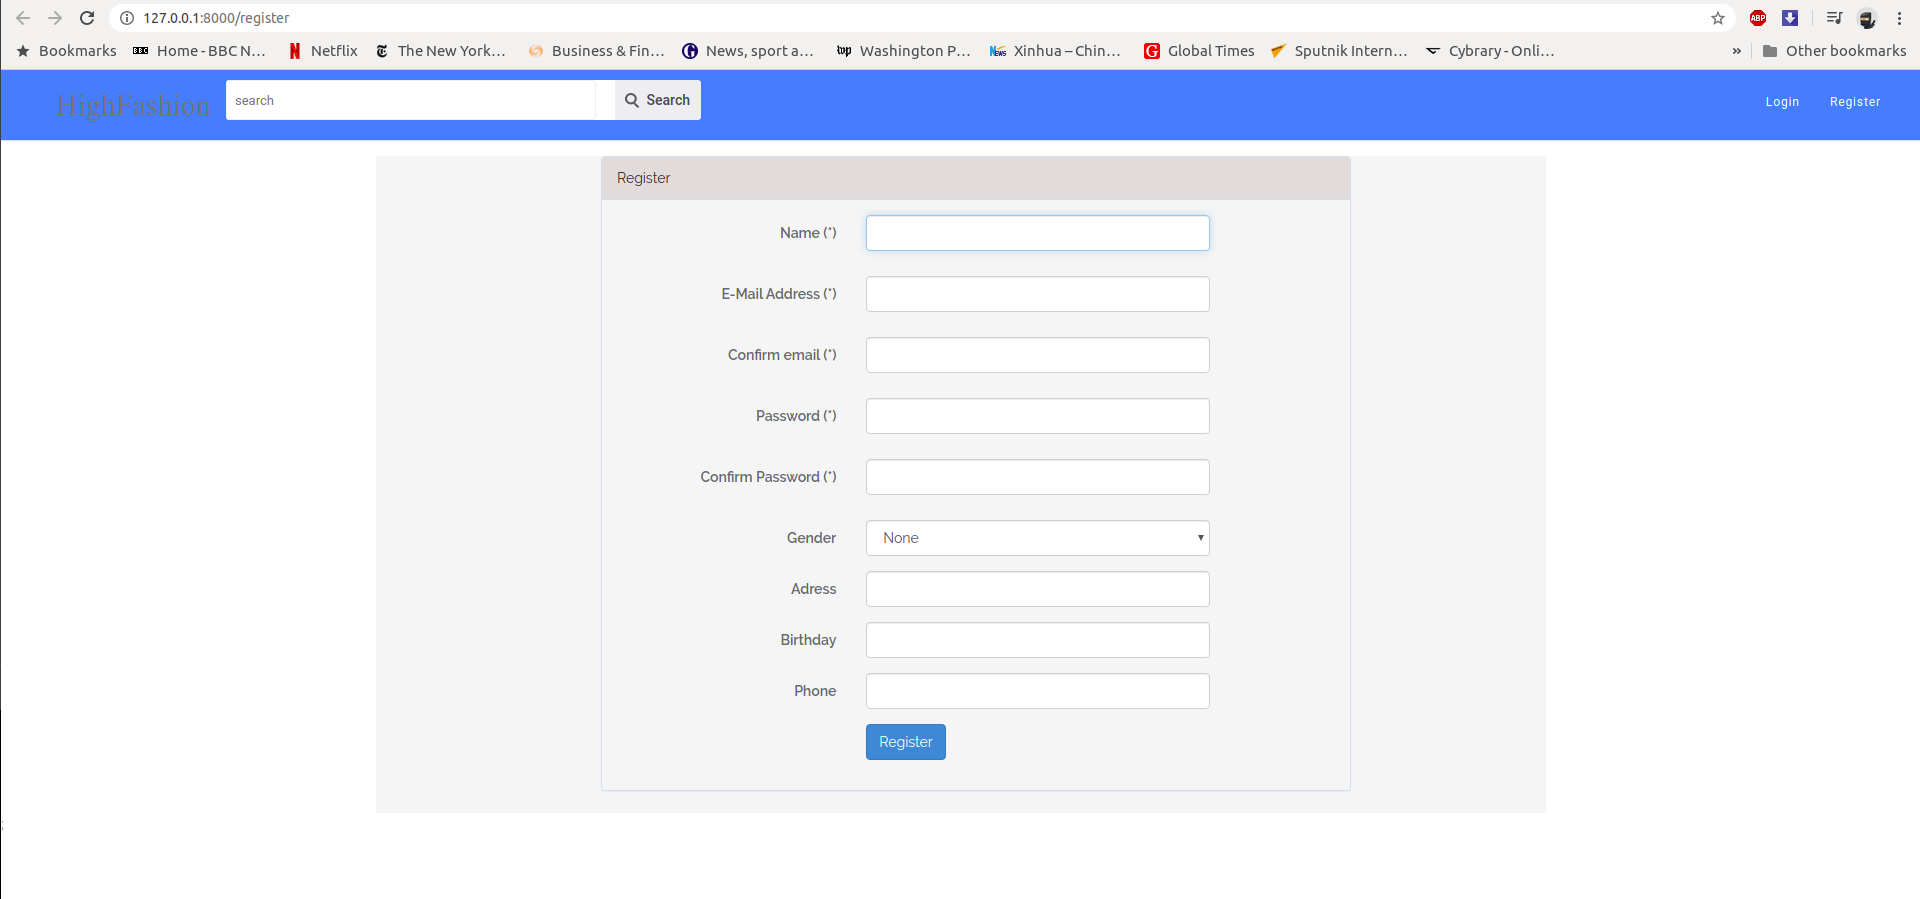
\includegraphics[scale=0.2]{figures/inreg.png}
	\caption{Giao diện đăng ký}
	\label{fig:inreg}
\end{figure}


Logic cho người dùng đăng ký được mô tả như sau. Đầu tiên, người dùng phải chọn chức năng đăng ký thành viên. Sau đó hệ thống sẽ mở ra giao diện để đăng ký cùng với các hộp thoại để người dùng điền các thông tin như "tên đăng nhập", "mật khẩu", "địa chỉ email" và các thông tin khác như "ngày sinh", "Công việc",... Mỗi bước người dùng nhập thông tin, hệ thống sẽ kiểm tra độ hợp lệ của thông tin. Cuối cùng người dùng đồng ý với các điều khoản của cửa hàng và gửi thông tin lên hệ thống. Hệ thống sẽ kiểm tra tất cả thông tin, nếu có lỗi sẽ hiển thị lỗi ở giao diện và ngược lại sẽ kết thúc phần đăng ký. Biểu đồ hoạt động của phần đăng ký được minh họa ở hình \ref{fig:actreg}.

\begin{figure}[h]
	\centering
	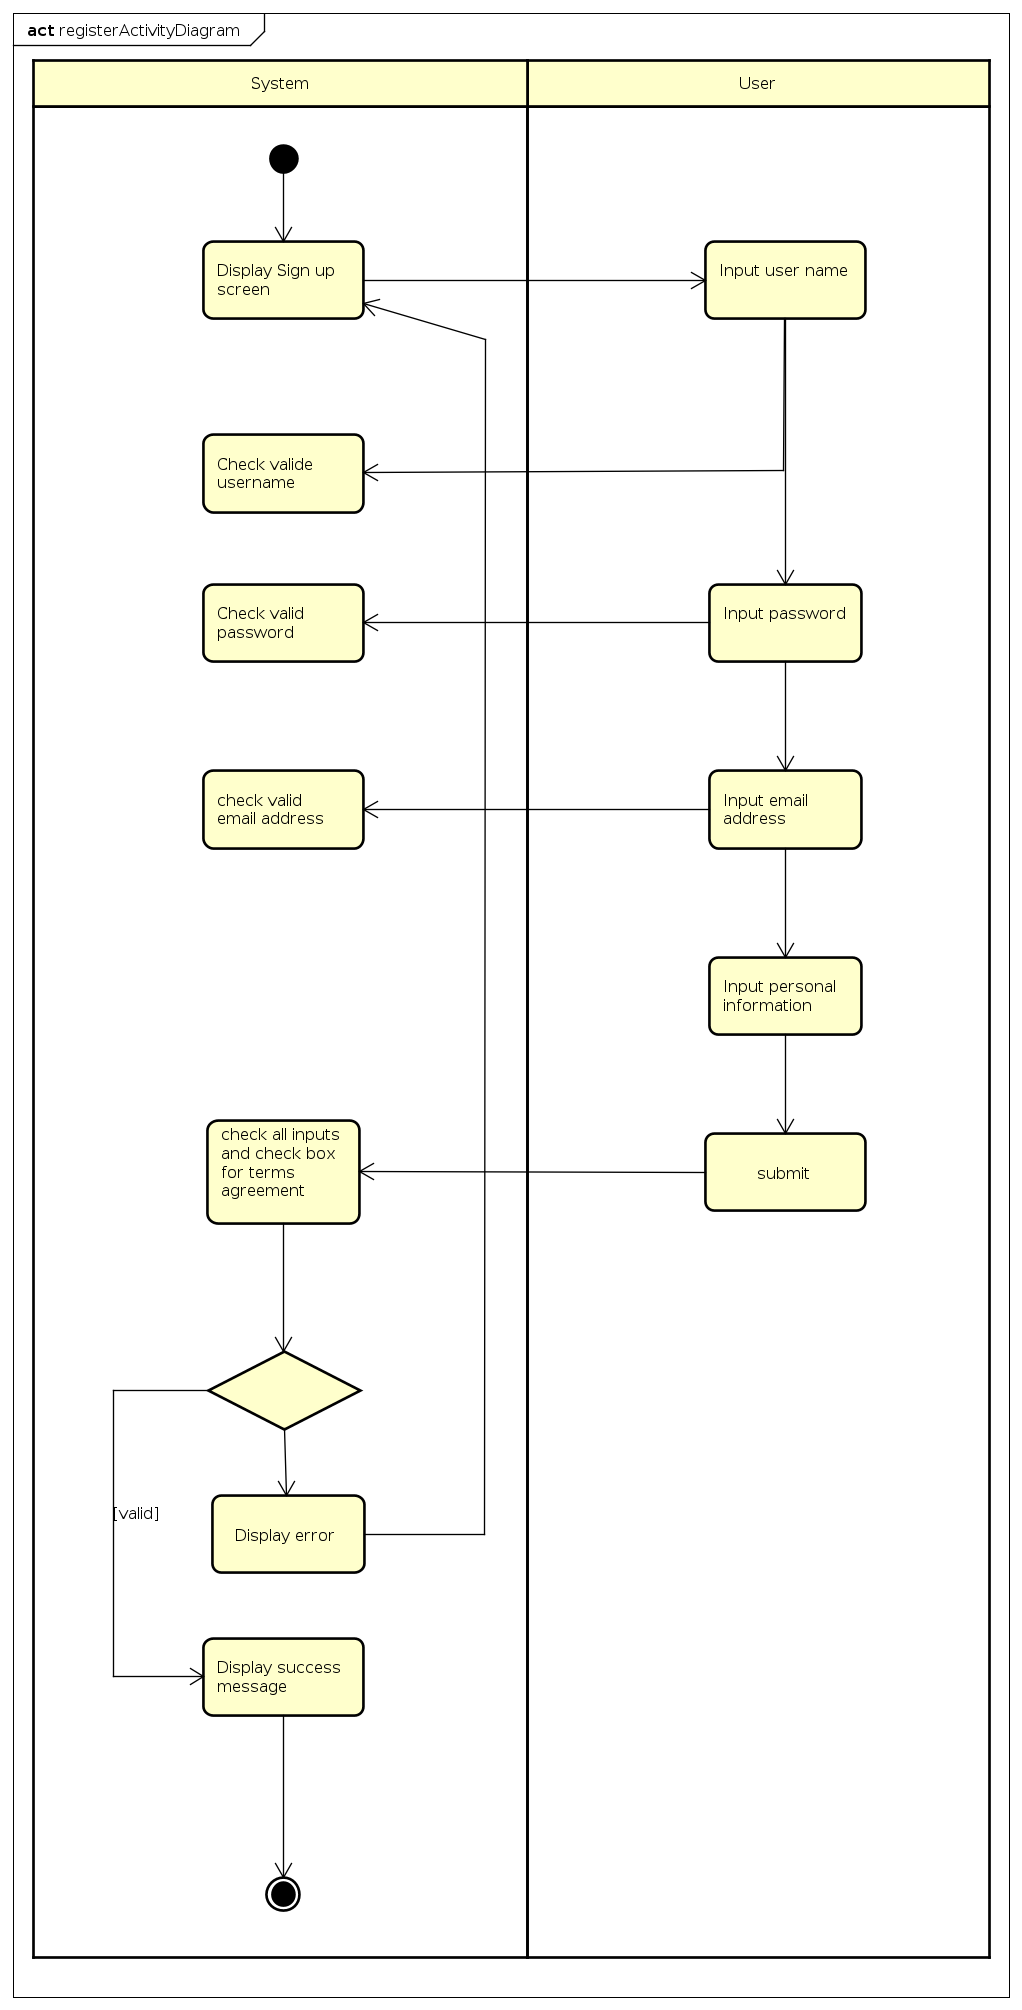
\includegraphics[scale=0.3]{figures/actreg.png}
	\caption{Biểu đồ hoạt động đăng ký người dùng}
	\label{fig:actreg}
\end{figure}

Sau khi người dùng đăng ký thành viên, thì người dùng có thể sử dụng tên đăng nhập và mật khẩu đã đăng ký để truy cập vào hệ thống. 

\subsection{Sprint 2: Module sản phẩm}

Kết thúc sprint đầu tiên sau khi đã được kiểm thử thành công, sprint thứ 2 được xây dựng hoàn  toàn độc lập với sprint đầu tiên. Cơ sở dữ liệu cho sản phẩm và loại sản phẩm được thêm vào cơ sở dữ liệu và được minh họa như trong hình \ref{fig:dataproduct}. 

\begin{figure}[h]
	\centering
	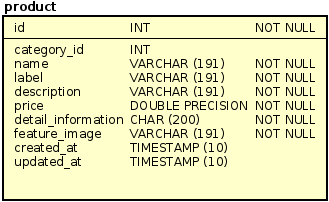
\includegraphics[scale=0.3]{figures/actproduct.png}
	\caption{Cơ sở dữ liệu cho sản phẩm}
	\label{fig:dataproduct}
\end{figure}

Ở module này, người dùng sẽ có thể tìm kiếm sản phẩm,  xem và tìm kiếm sản phẩm. Với chức năng tìm kiếm sản phẩm. Người dùng sẽ nhập từ khóa và hệ thống sẽ tìm kiếm từ khóa này trong cơ sở dữ liệu sản phẩm . Sau đó các sản phẩm tương thích với từ khóa nhập vào sẽ được hiển thị trên màn hình. Sơ đồ hoạt động được minh họa ở hình \ref{fig:actsearch}. 

\begin{figure}[h]
	\centering
	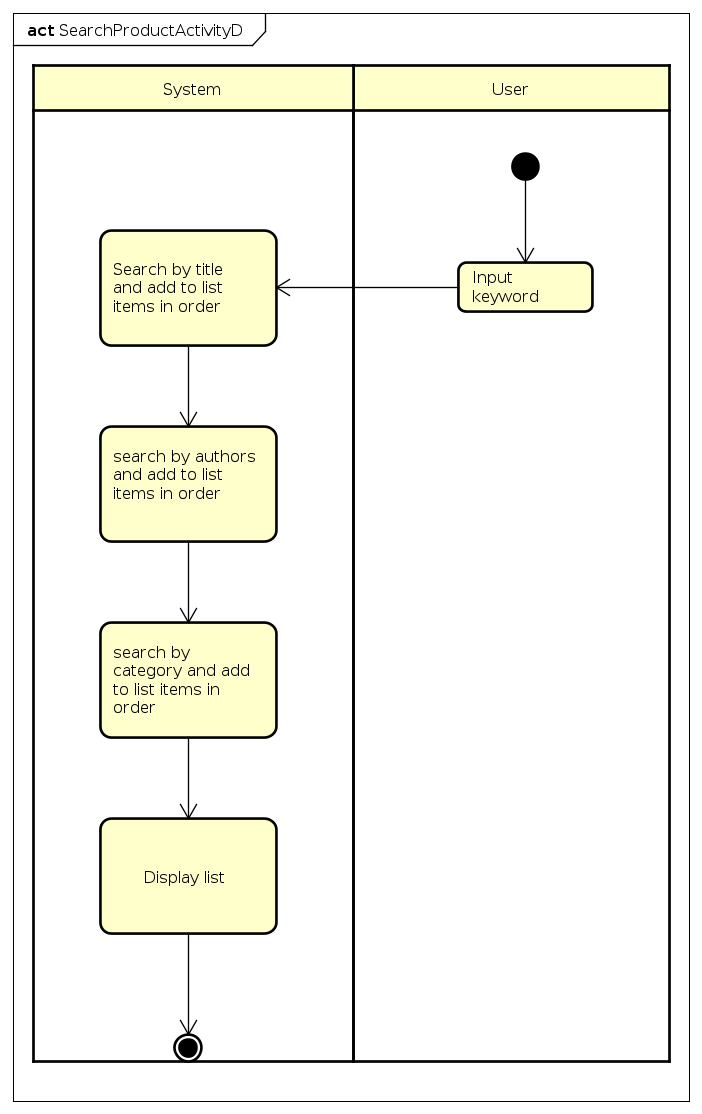
\includegraphics[scale=0.3]{figures/actsearch.png}
	\caption{Biểu đồ hoạt động tìm kiếm}
	\label{fig:actsearch}
\end{figure}

\begin{figure}[h]
	\centering
	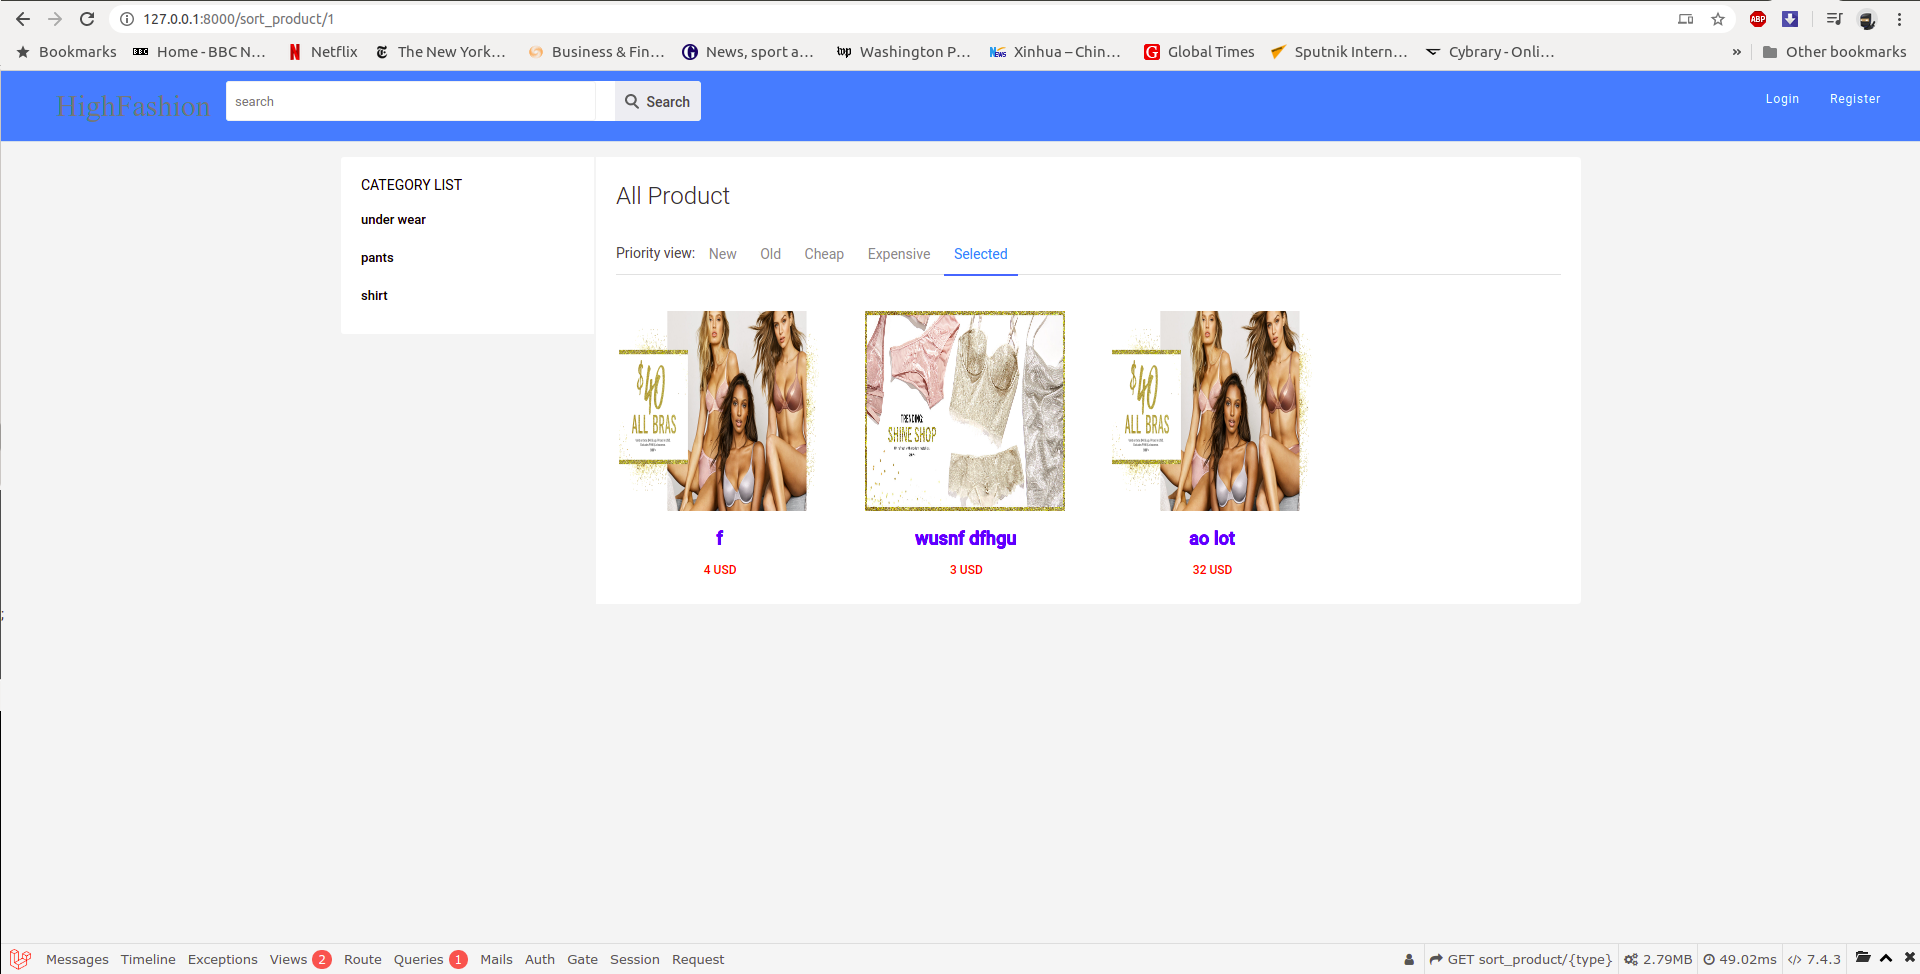
\includegraphics[scale=0.2]{figures/insort.png}
	\caption{Giao diện sắp xếp}
	\label{fig:insort}
\end{figure}

Tiếp đến với chức năng sắp xếp, xem sản phẩm thì người dùng lựa chọn xem sản phẩm được sắp xếp theo phân loại, theo giá cả hoặc theo năm phát hành. Biểu đồ hoạt động của chức năng này trình bày ở hình \ref{fig:actview}.

Như vấy spint thứ hai được xây dựng độc lập so với sprint đầu tiên. Phát triến sprint thứ hai không gây lỗi hoặc các vấn đề liên quan đến sprint thứ nhất. 

Từ cách thiết kế và xây dựng này các chức năng còn lại cũng được hoàn thiện. 

\begin{figure}[h]
	\centering
	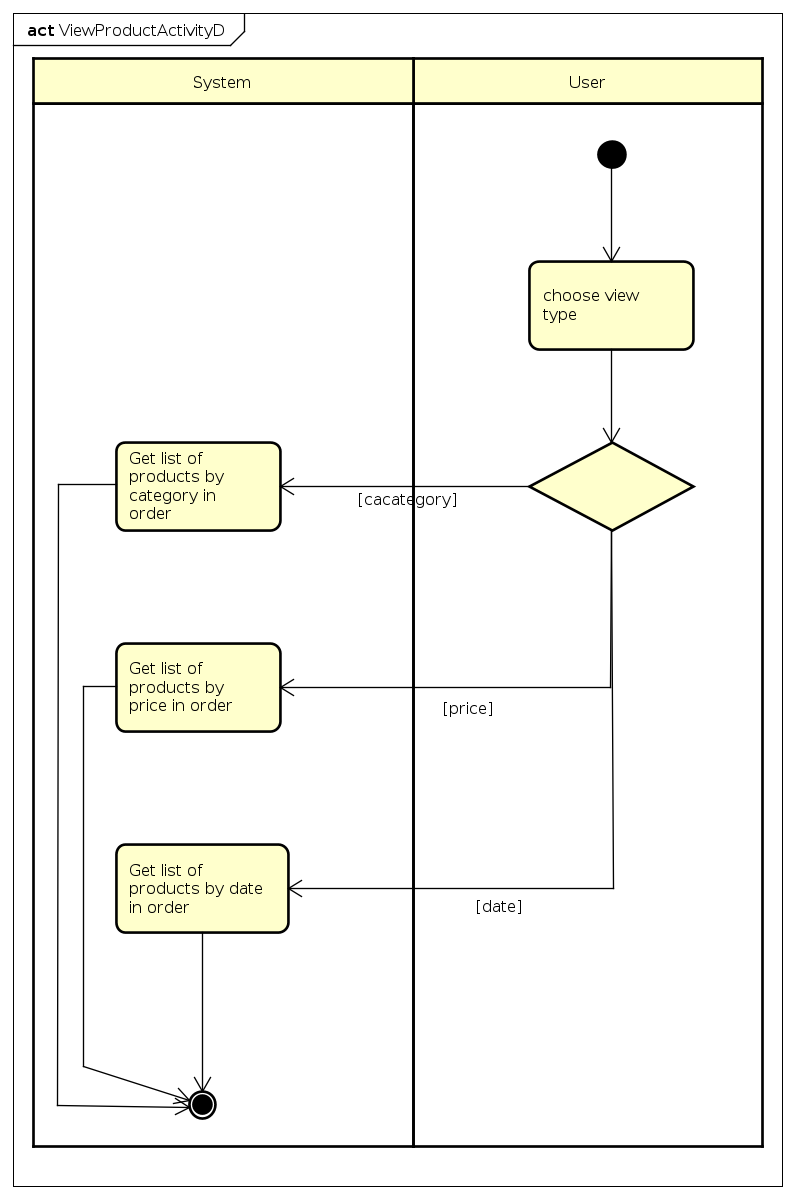
\includegraphics[scale=0.3]{figures/actview.png}
	\caption{Biểu đồ hoạt động sắp xếp sản phẩm}
	\label{fig:actview}
\end{figure}


\section{Kết luận}

Bài báo cáo đưa ra các tính chất, yêu cầu cần có của phần mềm. Bên cạnh đó, các mô hình phát triển phần mềm được nêu ra tỏng báo cáo bao gồm waterfall, V-shaped và spiral. Nội dung của báo cáo tập trung vào mô hình agile, trong đó khai thác kỹ hai phương pháp phổ biến nhất là Scrum và Extreme programming. Phần tiếp đó, báo cáo đưa ra ví dụ về việc áp dụng agile vào phát triển một sản phẩm trang web bán hàng online. 
Link project: \url{https://github.com/dnquang1996vn/sellingwear}



\printbibliography

%----------------------------------------------------------------------------------------


\end{document}